\documentclass[tikz,border=10pt]{standalone}
\begin{document}
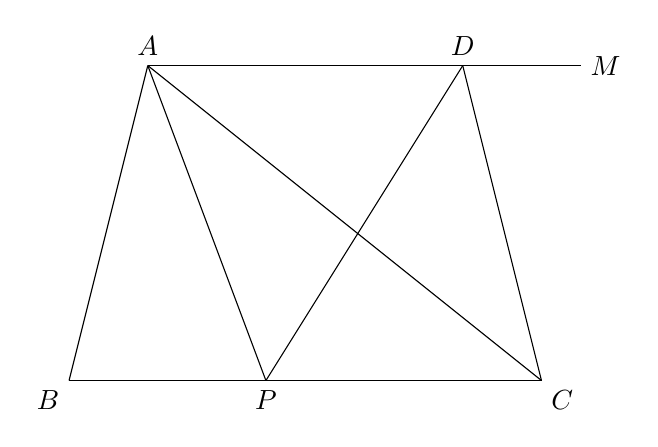
\begin{tikzpicture}
    \coordinate (B) at (0,0);
    \coordinate (C) at (6,0);
    \coordinate (P) at (2.5,0);
    \coordinate (A) at (1,4);
    \coordinate (D) at (5,4);
    \coordinate (M) at (6.5,4);

    \draw (A) -- (B);
    \draw (B) -- (C);
    \draw (C) -- (D);
    \draw (A) -- (M);
    \draw (A) -- (P);
    \draw (D) -- (P);
    \draw (A) -- (C);

    \node[above] at (A) {$A$};
    \node[below left] at (B) {$B$};
    \node[below] at (P) {$P$};
    \node[below right] at (C) {$C$};
    \node[above] at (D) {$D$};
    \node[right] at (M) {$M$};
\end{tikzpicture}
\end{document}
